%Dokumentklasse

%draft als optionohne bilder für bessere performance
%\documentclass[a4paper,12pt,]{scrreprt}

%normal mit Bildern
\documentclass[
a4paper,
12pt,
draft=True]
{scrartcl}

%Section als Chapter
\RedeclareSectionCommand[%
%beforeskip = -1sp plus -1sp minus -1sp,% kleinster negativer Wert, um den Absatzeinzug nach der Überschrift zu verhindern.
afterskip = 1.5 \baselineskip plus -1sp minus 1sp,
font = \Huge,
]{section}

\usepackage[left= 3cm,right = 3cm, bottom = 3cm,top = 3cm]{geometry}
%\usepackage[onehalfspacing]{setspace}

% ============= Packages =============
% Dokumentinformationen
\usepackage[
pdftitle={Praktikum - Umwelttechnik},
pdfsubject={},
pdfauthor={Roman-Luca Zank},
pdfkeywords={},	
%Links nicht einrahmen
hidelinks
]{hyperref}

%nur Text zum prüfen des Umfangs

% Standard Packages
%\usepackage[bottom]{footmisc}
\usepackage[utf8]{inputenc}
\usepackage[ngerman]{babel}

\usepackage[T1]{fontenc}
%\usepackage{helvet}

%\renewcommand{\familydefault}{\sfdefault}

\usepackage{graphicx}
\graphicspath{{img/}}
\usepackage{mhchem}
\usepackage{fancyhdr}
\usepackage{lmodern}
\usepackage{color}
\usepackage{placeins}
\usepackage{booktabs}
\usepackage{caption}
\usepackage[list=true]{subcaption}
\usepackage{longtable}
\usepackage{tikz}
\usepackage{pgfplots}
\usepackage{lastpage}
%\usepackage{ulem}
\usepackage{mathtools}
\usepackage{adjustbox}
\usetikzlibrary{patterns}
\usepackage{pdfpages}

%Einheitenpackage
\usepackage{siunitx}  
\sisetup{	locale = DE, 
	per-mode=fraction,
	inter-unit-product=\ensuremath{\cdot},
	detect-weight = true,
	quotient-mode=fraction
}
%neue Einheiten definieren
\DeclareSIUnit\xyz{xyz}	
\DeclareSIUnit\rpm{rpm}	
\DeclareSIUnit\mws{mWS}	
\DeclareSIUnit\degrees{^\circ}	

%Automatisch cdot statt *
\DeclareMathSymbol{*}{\mathbin}{symbols}{"01}


%Tabelle
\usepackage{tabularx}
\usepackage{tabulary}

%nur letzte Zeile der Gleichung nummerieren
\makeatletter
\def\Let@{\def\\{\notag\math@cr}}
\makeatother

% zusätzliche Schriftzeichen der American Mathematical Society
\usepackage{amsfonts}
\usepackage{amsmath}

%Abkürzungsverzeichnis
\usepackage{acronym}

%kein Abstand bei neuem Kapitel vom Seitenanfang
%\vspace*{2.3\baselineskip} = ORIGINAL
%\renewcommand*{\chapterheadstartvskip}{\vspace*{.0\baselineskip}}

%nicht einrücken nach Absatz
\setlength{\parindent}{0pt}

\urlstyle{same}


% ============= Kopf- und Fußzeile =============
\pagestyle{fancy}
%
\lhead{}
\chead{}
\rhead{}%\slshape }%\leftmark}
%%
\lfoot{}
\cfoot{}
\rfoot[{\thepage\ of \pageref*{LastPage}}]{Seite \thepage\ von \pageref*{LastPage}}
%%
\renewcommand{\headrulewidth}{0pt}
\renewcommand{\footrulewidth}{0pt}
%\renewcommand{\chapterpagestyle}{fancy}

%Fußnotelinie
%\let\footnoterule

%Fußnote mit Klammer
\renewcommand*{\thefootnote}{(\arabic{footnote})}

%Abb. statt Abbildung
\addto\captionsngerman{%
	\renewcommand{\figurename}{Abb.}%
	\renewcommand{\tablename}{Tab.}%
}

% ============= Package Einstellungen & Sonstiges ============= 
%Besondere Trennungen
%\hyphenation{De-zi-mal-tren-nung}
\usepackage[none]{hyphenat}
\hyphenpenalty=5000
\tolerance=5000
\providecommand\phantomsection{}

\usepackage{mathtools}


% ============= Dokumentbeginn =============

\begin{document}
%Seiten ohne Kopf- und Fußzeile sowie Seitenzahl
\pagestyle{empty}

%\begin{center}
\begin{tabular}{p{\textwidth}}


\begin{center}

\includegraphics[scale=0.75]{logos.jpg}\\
\end{center}


\\

\begin{center}
\LARGE{\textsc{
Protokoll \\
Analytik\\
}}
\end{center}

\\

%\begin{center}
%\large{Fakultät für Muster und Beispiele \\
%der Hochschule Musterhausen \\}
%\end{center}
%
%\\
\begin{center}
	\textbf{\LARGE{Versuch 2.2}}
\end{center}
\begin{center}
\Large{Nachweis und Bestimmung von Blei in Trinkwasser (Polarographie)}
\end{center}

\begin{center}
	\large{Gruppe 2.4 (BCUC4)}
\end{center}


\\
%\begin{center}
%zur Erlangung des akademischen Grades\\
%Bachelor of Engineering
%\end{center}


%\begin{center}
%vorgelegt von
%\end{center}

\begin{center}
\Large{\textbf{Teilnehmer:}} \\ 
\end{center}
\begin{center}
\large{Willy Messerschmidt \\
	Roman-Luca Zank} \\
\end{center}


\\

\begin{center}
\begin{tabular}{lll}
\large{\textbf{Protokollführer:}} & & \large{NAME}\\
&&\\
\large{\textbf{Datum der Versuchsdurchführung:}}&& \large{18.05.2020}\\
&&\\
\large{\textbf{Abgabedatum:}}&& \large{01.06.2020}
\end{tabular}
\end{center}

\\ \\ \\ \\
\large{Merseburg den \today}

\end{tabular}
\end{center}


%\include{14_danksagungen}

%\include{15_zusammenfassung}

% Beendet eine Seite und erzwingt auf den nachfolgenden Seiten die Ausgabe aller Gleitobjekte (z.B. Abbildungen), die bislang definiert, aber noch nicht ausgegeben wurden. Dieser Befehl fügt, falls nötig, eine leere Seite ein, sodaß die nächste Seite nach den Gleitobjekten eine ungerade Seitennummer hat. 
\cleardoubleoddpage

% Pagestyle für Titelblatt leer
\pagestyle{empty}

%Seite zählen ab
\setcounter{page}{0}

%Titelblatt
\begin{center}
\begin{tabular}{p{\textwidth}}


\begin{center}

\includegraphics[scale=0.75]{logos.jpg}\\
\end{center}


\\

\begin{center}
\LARGE{\textsc{
Protokoll \\
Analytik\\
}}
\end{center}

\\

%\begin{center}
%\large{Fakultät für Muster und Beispiele \\
%der Hochschule Musterhausen \\}
%\end{center}
%
%\\
\begin{center}
	\textbf{\LARGE{Versuch 2.2}}
\end{center}
\begin{center}
\Large{Nachweis und Bestimmung von Blei in Trinkwasser (Polarographie)}
\end{center}

\begin{center}
	\large{Gruppe 2.4 (BCUC4)}
\end{center}


\\
%\begin{center}
%zur Erlangung des akademischen Grades\\
%Bachelor of Engineering
%\end{center}


%\begin{center}
%vorgelegt von
%\end{center}

\begin{center}
\Large{\textbf{Teilnehmer:}} \\ 
\end{center}
\begin{center}
\large{Willy Messerschmidt \\
	Roman-Luca Zank} \\
\end{center}


\\

\begin{center}
\begin{tabular}{lll}
\large{\textbf{Protokollführer:}} & & \large{NAME}\\
&&\\
\large{\textbf{Datum der Versuchsdurchführung:}}&& \large{18.05.2020}\\
&&\\
\large{\textbf{Abgabedatum:}}&& \large{01.06.2020}
\end{tabular}
\end{center}

\\ \\ \\ \\
\large{Merseburg den \today}

\end{tabular}
\end{center}
 %Prokolle
%\begin{center}
\begin{tabular}{p{\textwidth}}


\begin{center}

\includegraphics[scale=0.75]{img/logos.jpg}\\
\end{center}


\\

\begin{center}
\LARGE{\textsc{
Recherche \\
Rückgewinnung von Ammoniak aus Industrieabwässern\\
}}
\end{center}

%\begin{center}
%\large{Fakultät für Muster und Beispiele \\
%der Hochschule Musterhausen \\}
%\end{center}
%
%\\
 \\
 
\begin{center}
\textbf{\Large{Seminararbeit in Medienrecherche}}
\end{center}

\begin{center}
	\large{im WiSe 2019}
\end{center}
 \\
%\begin{center}
%zur Erlangung des akademischen Grades\\
%Bachelor of Engineering
%\end{center}


\begin{center}
\large{vorgelegt von}
\end{center}
\\


\begin{center}
\Large{\textbf{Roman-Luca Zank}} \\
\end{center}

\begin{center}
3. Semester \\
Chemie- und Umwelttechnik \\
\end{center}


\begin{center}
\begin{tabular}{lll}
	\textbf{E-Mail:} & & romanzank@mail.de\\
	\textbf{Matrikelnummer:} & &25240\\
	\textbf{Adresse:} & &Platz der Bausoldaten 2, Zimmer 224\\
	\textbf{Ort:} & &06217 Merseburg\\
	&& \\
	\textbf{Prüfer:} & & Dr. Frank  Baumann\\
\end{tabular}
\end{center}

\\ \\ \\ \\ \\
\large{Merseburg, \today}

\end{tabular}
\end{center}
 %Seminar-/Abschlussarbeit

% Pagestyle für Rest des Dokuments
\pagestyle{fancy}

%Inhaltsverzeichnis
\tableofcontents
\thispagestyle{empty}

%Inhalt
%
%Verzeichnis aller Bilder
\label{sec:bilder}
\listoffigures
\addcontentsline{toc}{chapter}{Abbildungsverzeichnis}
\thispagestyle{empty}

%Verzeichnis aller Tabellen
\label{sec:tabellen}
\listoftables
\addcontentsline{toc}{chapter}{Tabellenverzeichnis}
\thispagestyle{empty}



%%Abkürzungsverzeichnis
%\setlength{\columnsep}{20pt}
%\twocolumn
%\addchap{Nomenklatur}
%\label{sec:abkurzung}
%\begin{acronym}
%\acro{kf}[$\text{k}_\text{f}$]{Durchlässigkeitsbeiwert}
%\acro{t}{Durchlaufzeit}
%\acro{tm}[$\text{t}_\text{m}$]{Mittlere Durchlaufzeit}
%\acro{V}{Volumen}
%\acro{h}{Höhe der Wassersäule}
%\acro{Q}{Volumenstrom}
%\acro{l}{Durchströmte Länge}
%\acro{A}{Grundfläche}
%\acro{d}{Durchmesser}
%
%\end{acronym}
%\subsubsection{Aufrufen einer Abkürzung}
%\acs{rT}
%\begin{verbatim}
%\acs{Abkürzung}
%\end{verbatim}

\section{Einleitung}
\label{sec:einleitung}
%Beschreibung der Grundzüge der Polarographie

Als Teil der Voltammetrie bezeichnet die Polarographie ein Analyseverfahren, bei dem eine tropfende Quecksilberelektrode als polarisierbare Elektrode genutzt wird (siehe Abb. \ref{fig:schema_polarograph}). Die im Praktikum aufgenommenen Daten beinhalten die \mbox{Stromstärke $I$} als Messgröße über die angelegte \mbox{Gleichspannung $U$} als variierende Größe. Das Verfahren beruht dabei auf der elektrolytischen Abscheidung, in diesem Fall Reduktion, von Stoffen aus der Probenlösung.\cite{Brehm.2004}

%Start
\begin{figure}[h!]
	\centering
	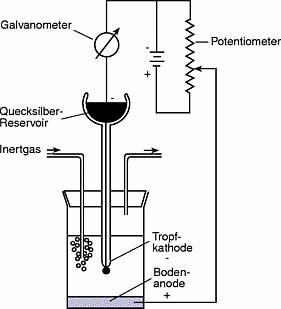
\includegraphics[width=0.4\textwidth]{img/Polarograph}
	\caption{Schematische Darstellung eines Polarographen \cite{Brehm.2004}}
	\label{fig:schema_polarograph}
\end{figure}
\FloatBarrier
%Ende

Im Versuch wurde mittels des Analyseverfahrens der Polarographie, der Bleigehalt in einer unbekannten Wasserprobe bestimmt.

\section{Theorie}
\label{sec:theorie}

\subsection{Voltammetrie}
Voltammetrie ist eine Sammelbezeichnung für einige elektrochemische Analysemethoden, bei denen die Spannung (das Potential) und der fließende Strom zwischen mindestens zwei Elektroden betrachtet werden, um daraus Aussagen zur Zusammensetzung einer Probe abzuleiten.\\
Die \textit{Voltammetrie} ist nicht mit der \textit{Voltametrie} zu verwechseln. Bei letzterer wird lediglich die Spannung gemessen.
\subsection{Die Elektrochemische Spannungsreihe}


Die Elektrochemische Spannungsreihe ordnet Metalle nach ihrem elektrochemischen Potential. Als Bezug dient dabei stets die Standardwasserstoffelektrode. In Verbindung letzterer Halbzelle mit einem Metall, in seiner einmolaren Metallsalzlösung bei Standardbedingungen, kann das Standardpotential des Metalls als anliegende Spannung zwischen den Elektroden gemessen werden. Das Vorzeichen der Standardpotentiale sagt aus, in welche die Richtung Elektronen strömen. Es besteht ein direkter Zusammenhang zwischen dem Standardelektrodenpotential eines Metalls und dessen Bestreben reduziert zu werden. Je größer das Elektrodenpotential ist, umso edler ist auch das Metall und umso eher wird es reduziert. Verwendung findet dieser Umstand zum Beispiel in der Berechnung galvanischer Elemente. Im folgenden kann anhand der Standardelektrodenpotentiale gelöster Metallionen deren Positionierung in einem Polarogramm abgeleitet werden.\cite{spannungsreihe}\\

\vline

\subsection{Analyse der Polarogramme}
Grundlage für die Analyse der enthaltenen Metall-Ionen ist die aufgenommene Strom-Spannungs-Kurve des Polarographen. Aufgrund der spezifischen Halbstufenpotentiale von Metall-Ionen ändert sich bei unterschiedlichen Arbeitspotentialen die gemessene Stromstärke. Dieser Strom an der Arbeitselektrode 
tritt als Folge der Reduktionsreaktion der Metall-Ionen auf und ist direkt proportional zur Konzentration des umgesetzten Stoffes. Der Strom im Zusammenhang mit diesem Massentransport der Ionen wird als \textsc{Faraday}scher Strom bezeichnet. \linebreak Um eine ausreichende Leitfähigkeit und somit einen entsprechenden Ladungstransport in der Lösung garantieren zu können, werden den untersuchten Proben oft Grundelektrolyten in Form von Salzen, Säuren oder Basen zugegeben.\linebreak
Aufgrund der spezifischen Halbstufenpotentiale lassen sich qualitative Ergebnisse dieses Verfahrens auswerten. Betrachtet man jedoch auch den Zusammenhang des Stromflusses bei einem bestimmten Arbeitspotential mit der Konzentration des umgesetzten Stoffes, so lassen sich ebenfalls quantitative Bewertungen äußern.\linebreak
Für diese Betrachtung ist jedoch eine Form der Kalibrierung notwendig, um die gemessenen Signale quantitativ auswerten zu können. Dies ist zum einen über einen externen oder internen Standard möglich, jedoch wurde sich aufgrund der geringen zu bestimmenden Konzentrationen in diesem Versuch für die Aufstockmethode, auch Standardadditionsmethode genannt, entschieden. Möchte man einen internen oder externen Standard nutzen so sind in diesem Fall ebenfalls Kalibrierkurven mit linearem Zusammenhang mittels bekannter Referenz aufzustellen.\linebreak
Bei dieser Methode wird in diesem Versuch nach der polarographischen Analyse der unbehandelten Probe, eine definierte Menge eines bekannten Standards zugegeben. Dieser Standard enthält dabei den zu bestimmenden Stoff in einer exakt bekannten Konzentration. Aus den gemessenen Datenpunkten lässt sich nun eine Geradengleichung bestimmen (siehe Abb. \ref{fig:standardaddition} und Gl. \ref{gl:1}).

\begin{flalign}
\label{gl:1}
Y &= \frac{\Delta y}{\Delta x}*X+yA
\end{flalign}

%Start
\begin{figure}[h!]
	\centering
	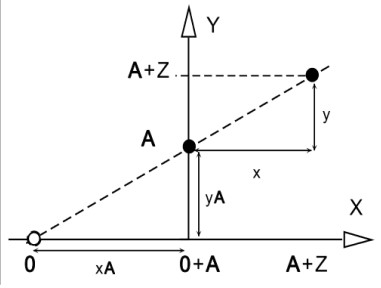
\includegraphics[width=0.5\textwidth]{img/Standardaddition}
	\caption{Darstellung der Standardadditionsmethode \cite{}}
	\label{fig:standardaddition}
\end{figure}
\FloatBarrier
%Ende

Aus der ermittelten Geradengleichung, lässt sich nun, aufgrund der geometrischen Beziehung der Strahlensätze, die Konzentration der Probe über den Wert $xA$ in Abb. \ref{fig:standardaddition} bestimmen. Eine Herleitung dazu ist unter Gl. \ref{gl:2} und Gl. \ref{gl:3} zu finden. Die Bedeutungen der Variablen sind nachfolgend in der Tabelle \ref{tab:variablen} aufgeführt.

\begin{flalign}
\label{gl:2}
	Y &= \frac{y}{x}*X+yA\\
	X&= \frac{Y-yA}{\frac{y}{x}}
\end{flalign}

\textit{Für $Y=0$ heißt das:}

\begin{flalign}
\label{gl:3}
X&= xA = \frac{0-yA}{\frac{y}{x}} = \frac{-yA}{\frac{y}{x}}\\
xA&= -c\\
c	&= \underline{\underline{\frac{yA}{\frac{y}{x}}}}
\end{flalign}

\vspace*{-5mm}

%Tabelle START
\renewcommand{\arraystretch}{1.2}
\begin{table}[h!]
	\centering
	%\caption{Variablen der Abb.\ref{fig:standardaddition} und der Tab.\ref{tab:variablen} und ihre Bedeutungen}
	\caption{Variablen und ihre Bedeutung}
	\label{tab:variablen}
	%\makebox[\textwidth]{
	%	\resizebox{17cm}{!}{
			\begin{tabular}{c|c}
				\hline
				\textbf{Variable}&\textbf{Bedeutung} \\
				\hline
				A& Analyt \\
				Z& Zugabe\\
				$Y$& Signalwert\\
				$yA$& Signalwert der Testlösung - nur Analyt\\
				$\Delta y$& Signaländerungnach Zugabe der Standardlösung \\
				$X$& Analytwert\\
				$xA$&Analytkonzentration in der Testlösung\\
				$\Delta x$& Konzentrationsändeung durch Standard-Zugabe \\
				\hline	
			\end{tabular}
		%	}
			%}
		\end{table}
		\FloatBarrier
		\vspace*{-2.5mm}
		%Tabelle Ende


\newpage
\section{Geräte und Chemikalien}
\label{sec:geraete}

\textbf{Geräte:}
\begin{itemize}
	\item VA Computrace System 757 (\textsc{Fa. Metrohm, Schweiz})
	\item Druckbehälter mit Stickstoff
	
\end{itemize}

\vspace*{5mm}

\textbf{Proben/Chemikalien:}
\begin{itemize}
	\item zu untersuchende Wasserprobe
	\item \ce{HNO3}, ultrarein, zur Konservierung von Wasserproben, evtl. auch zur Herstellung von Standardlösungen
	\item Stickstoff als Spülgas zur Entlüftung (Beseitigung von Sauerstoff)
	\item Leitelektrolyt: Acetatpuffer, pH$=4,64 \quad \left(\SI{1}{\mol\per\liter}\right)$
	\item Triton-X (als Netzmittel)
	\item Multielementcocktail mit \ce{Zn}-,\ce{Cd}-,\ce{Pb}-,\ce{Cu}-Konzentrationen von je \SI{250}{\milli \gram\per \liter}
	\item Blei-Standardlösung mit $\beta(\ce{Pb^{2+}})=\SI{1}{\gram\per\liter}$
\end{itemize}







\section{Durchführung}
\label{sec:durchfuerung}
\subsection{Versuchsteil 1: Aufnahme und Glättung des Polarogramms}
Nach Starten des Computersystems mit der Software \textsc{757 VA Computrace} werden die entsprechenden Voreinstellungen des Systems nach der Versuchsanleitung getroffen. Während dessen werden \SI{10}{\milli \liter} des Acetat-Puffer mit \SI{1}{\mol\per \liter} mit deionisierten Wasser auf \SI{100}{\milli \liter} zu \SI{0,1}{\mol\per \liter} aufgefüllt (vgl. mit Gl. \ref{gl:4}).
\begin{flalign}
\label{gl:4}
	n_{\text{vorher}}(\text{Acetatpuffer}) &= 	n_{\text{nachher}}(\text{Acetatpuffer})\\[2mm]
	c_{\text{vorher}}(\text{Acetatpuffer})*V_{\text{vorher}}(\text{Acetatpuffer}) &= c_{\text{nachher}}(\text{Acetatpuffer})*V_{\text{nachher}}(\text{Acetatpuffer})\\[2mm]
	c_{\text{nachher}}(\text{Acetatpuffer})&=\frac{V_{\text{vorher}}(\text{Acetatpuffer})}{V_{\text{nachher}}(\text{Acetatpuffer})}*c_{\text{vorher}}(\text{Acetatpuffer})\\[2mm]
	&=\frac{\SI{10}{\milli \liter}}{\SI{100}{\milli \liter}}*\SI{1}{\mol \per \liter}\\[2mm]
	&= \underline{\underline{\SI{0,1}{\mol \per \liter}}}											
\end{flalign} 

\newpage

In Folge der Verdünnung des Acetat-Puffers werden davon \SI{25}{\milli \liter} in das Messgefäß pipettiert, sowie weitere \SI{10}{\micro\liter} Triton-X, um die Oberflächenspannung der Lösung zu reduzieren. Die Messung durch das Messgerät wird mittels Mausklick gestartet und gibt ein Polarogramm aus.\\ 
Als nächster Schritt im Versuch wird versucht mittels fünfminütigen Spülens mit Stickstoff den gelösten Sauerstoff zu beseitigen. Ziel ist es dabei das zuvor ausgegebene Polarogramm zu glätten. \\
Zuletzt werden in diesem Versuchsteil \SI{1000}{\micro \liter} des Multielementcocktails mit je \SI{25}{\gram \per\liter} zugesetzt und ebenfalls ein Polarogramm davon aufgenommen.\\
Ein Vergleich und eine Auswertung der ausgegebenen Polarogramme erfolgt unter Abschnitt \ref{sec:ergebnisse}.

\subsection{Versuchsteil 2: Identifikation und Quantifizierung des Analyten Blei der Wasserprobe}
Die im Polarogramm gezeichneten Peaks entsprechen voraussichtlich den verschiedenen, enthaltenen Metall-Ionen im Messgefäß. Für die eindeutige Bestimmung des Peaks für Blei wird eine \SI{250}{\micro \liter} Blei-Standardlösung zugegeben. Die Peaks der restlichen Ionen bleiben gleich, während der Peak der für die Blei-Ionen steht, steigen wird. Die Peaks der jeweiligen Programme werden zum einen manuell und automatisch vom System bestimmt. Für nachfolgende Bestimmungen werden die Potentiale $E_{Start}$ und $E_{Ende}$ anhand des Peaks von Blei $\pm \SI{0,2}{\volt}$ festgelegt.\\
Die Konzentration des Analyten Blei wird im Folgenden mittels Standardadditionsmethode (beschrieben unter Abschnitt \ref{sec:theorie}) durch zweimaliges Aufstocken bestimmt.\linebreak
Dazu wird das Messgefäß gereinigt und der Maßkolben mit der Wasserprobe mit \SI{10}{\milli \liter} unverdünnter Pufferlösung $\left(\SI{1}{\mol\per\liter}\right)$ versetzt und mit destilliertem Wasser aufgefüllt. \SI{25}{\milli \liter} dieser Analysenprobe werden in das gereinigte Messgefäß mit \SI{10}{\micro\liter} Triton-X gegeben. Es werden nun die entsprechenden Parameter im Computerprogramm nach Praktikumsanleitung für zweimaliges Aufstocken mit \SI{200}{\micro\liter} Blei-Standard eingegeben. 
Die Messung startet ebenfalls per Mausklick und je nach Messfortschritt und Aufforderung des Programms wird der entsprechende Standard manuell zugegeben. Zum Schluss gibt das Programm die quantitativen, gemessenen Daten zusammengefasst in Graphen, Kalibriergeradengleichungen und Konzentration des Analyten aus.

\newpage


\section{Ergebnisse und Berechnungen}
\label{sec:ergebnisse}
\subsection{Versuchsteil 1: Aufnahme und Glättung des Polarogramms}
 
 %Start
 \begin{figure}[h!]
 	\centering
 	\includegraphics[width=1.0\textwidth]{img/Daten_farbig2}
 	\caption{Strom-Spannungskurven (Polarogramme) des Versuchsteils 1}
 	\label{fig:daten_farbig}
 \end{figure}
 \FloatBarrier
 %Ende   
   

 \begin{center}
 
 
 %Tabelle START
 \vspace*{-2.5mm}
 \renewcommand{\arraystretch}{1.2}
 \begin{threeparttable}[h!]
 	\centering
 	\caption{Zuordnung der Peaks den Elementen des Multielementcocktails}
 	\label{tab:peaks}
 %	\resizebox{17cm}{!}{
 	\begin{tabulary}{\textwidth}{|C|C|C|C|C|}
 		\hline
 		\textbf{Element} 	&  \textbf{Kupfer}  &\textbf{Blei}& \textbf{Cadmium} & \textbf{Zink}\\ 
 							&\ce{Cu}&\ce{Pb}&\ce{Cd}&\ce{Zn}\\
 		\hline
 		\textbf{E$^\circ$ \tnote{(1)} \quad[V]}&$+0,52$&$-0,13$&$-0,40$&$-0,76$\\
 		\hline
 		\textbf{Peak Nr.} 		&1&2&3&4\\
 		\hline
	 	\textbf{Potential [V]} &&&&\\
 		Manuell &0,04&-0,38&-0,55&-0,96\\
 		Automatisch &0,0369&-0,38&-0,552&-0,969\\
 		\hline
 	\end{tabulary}
 	%}
 		\begin{tablenotes}\footnotesize 
 					\item[(1)]Standardelektrodenpotential 
 				\end{tablenotes}
 \end{threeparttable}
 \FloatBarrier 
% \vspace*{-2.5mm}
 %Tabelle ENDE
\end{center}
\newpage
 Die Verwendung von Verhältnisgleichungen erlaubte ein sehr präzises, manuelles Ablesen aus dem Diagramm. Eine solche Verhältnisgleichung ist in Gl. (\ref{gl:verhaltnis}) beispielhaft dargestellt. Die Längenangaben in Millimetern werden durch das Anlegen eines Lineals an die Achsen auf dem Ausdruck des Diagramms erhalten. 
 \begin{flalign}\label{gl:verhaltnis}
 	\frac{\SI{76}{\milli\meter}}{\SI{-0,600}{\volt}}&=\frac{\SI{122}{\milli\meter}}{x}\\
 	x&=\underline{\SI{-0,963158}{\volt}}\approx\underline{\underline{\SI{-0,96}{\volt}}}
 \end{flalign}
Anschließend wurde noch sinnvoll gerundet.

 
 \subsection{Versuchsteil 2: Identifikation und Quantifizierung des Analyten Blei der Wasserprobe}
	
	\subsubsection*{Berechnung der Konzentration nach Aufstockung mit Bleistandard:}
	\begin{flalign}\label{gl:7}
	V_{\text{Standard-Zugabe}} * c_{\text{Standard-Zugabe}} &= V_{\text{Lösung}} * c_{\text{Lösung}}\\
	c_{\text{Lösung}} 	&= \frac{V_{\text{Standard-Zugabe}} }{V_{\text{Lösung}}} * c_{\text{Standard-Zugabe}}		
	\end{flalign}
	\begin{flalign}\label{gl:8}
	c_{\text{Lösung},1} &=\frac{\SI{200e-6}{\liter}}{\SI{25e-3}{\liter}} * \SI{1000}{\milli \gram \per \liter}\\
	&= \underline{\SI{8}{\milli \gram \per \liter}	}\\[3mm]
	c_{\text{Lösung},2} &=\frac{\SI{400e-6}{\liter}}{\SI{25e-3}{\liter}} * \SI{1000}{\milli \gram \per \liter}\\
	&= \underline{\SI{16}{\milli \gram \per \liter}	}
	\end{flalign}
	
	
	 %Tabelle START
	\vspace*{-2.5mm}
	\renewcommand{\arraystretch}{1.2}
	\begin{table}[h!]
		\centering
		\caption{Messwerte der Messreihe 1}
		\label{tab:messreihe1}
		%\resizebox{10cm}{!}{
		\begin{tabulary}{\textwidth}{C|CC}
			\hline
			\textbf{Konzentration der Bleizugabe in \si{\milli \gram \per \liter}} &  \textbf{Spannung in \si{\volt}}  &\textbf{Stromstärke in \si{\nano \ampere}}\\ 
			\hline
			0 	&-0,376	&-113,0	\\
			0 	&-0,376	&-112,5	\\
			8 	&-0,376	&-268,2	\\
			8 	&-0,376	&-266,6	\\
			16 	&-0,376	&-422,8	\\
			16 	&-0,382	&-416,0	\\
			\hline
		\end{tabulary}
		%}
	\end{table}
	\FloatBarrier
	\vspace*{-2.5mm}
	%Tabelle ENDE
	%Tabelle START
	\vspace*{-2.5mm}
	\renewcommand{\arraystretch}{1.2}
	\begin{table}[h!]
		\centering
		\caption{Messwerte der Messreihe 2}
		\label{tab:messreihe2}
		%\resizebox{10cm}{!}{
		\begin{tabulary}{\textwidth}{C|CC}
			\hline
			\textbf{Konzentration der Bleizugabe in \si{\milli \gram \per \liter}} &  \textbf{Spannung in \si{\volt}}  &\textbf{Stromstärke in \si{\nano \ampere}}\\ 
			\hline
			0 	&-0,382	&-129,3	\\
			0 	&-0,382	&-139,2	\\
			8 	&-0,382	&-286,2	\\
			8 	&-0,382	&-282,2	\\
			16 	&-0,382	&-425,1	\\
			16 	&-0,382	&-424,0	\\
			\hline
		\end{tabulary}
		%}
	\end{table}
	\FloatBarrier
	\vspace*{-2.5mm}
	%Tabelle ENDE
	
	\pagebreak

	\subsubsection*{Aufstellen der Kalibriergeraden:}
	Die Kalibriergerade wird manuell erstellt in dem die die gemessenen Stromstärken der Peaks über dem Konzentrationszuschuss durch die Zugabe der Blei Standardlösung aufgetragen werden. Die Stromstärken für die Y-Achse werden aus den gewonnenen Polarogrammen abgelesen. Hier treten Ablesefehler von etwa $\pm$ \SI{10}{\nano\ampere} auf. Die Konzentrationsänderung bei Addition von Standardlösung wird entsprechend der Gleichungen (\ref{gl:7}) und (\ref{gl:8}) berechnet. Mittels des Tabellenkalkulationsprogramms \textit{LibreOffice Calc} wurde eine lineare Regression zur Bestimmung der Kalibriergeradengleichung durchgeführt. Es ergaben sich folgende Funktionsgleichungen:
	$$f_1(x)=y=-19,166*x - 113,19 $$ 
	$$f_2(x)=y=-18,144*x - 135,85 $$ 
	
	\begin{figure}[h!]
		\begin{center}
			\resizebox{0.9\textwidth}{!}{
				\begin{tikzpicture}[trim axis left, trim axis right]
				\begin{axis}[
				axis lines = middle,
				width = 20cm,
				height = 11cm,
				xmin = -10,
				xmax = 20,
				%	ymin = -0.1,
				%	ymax = 0,
				%	ytick = {-4.5,-4,...,-1},
				xtick = {-10,-9,...,20},
				ylabel={Stromstärke in \si{\nano \ampere}},
				y label style={at={(0.25,0.40)}, rotate=90},
				xlabel={Konzentration der Blei-Standard-Zugabe in \si{\milli \gram \per \milli \liter}},
				legend style={at={(0.75,0.45)},anchor=west},
				y dir = reverse,
				]
				\addplot table {datenm1.dat};
				\addplot +[mark=none, dashed, black, domain=-10:20] {-19.166*x - 113.19};
				\addplot table {datenm2.dat};
				\addplot +[mark=none, dotted, black, domain=-10:20] {-18.144*x - 135.85};
				
				\legend{Messreihe 1, Regression Messreihe 1,Messreihe 2, Regression Messreihe 2};
				\end{axis}
				\end{tikzpicture}
			}
			\caption{Gemessene Stromstärken in Abhängigkeit von der Konzentration der Blei-Standardzugabe (siehe Tab. \ref{tab:messreihe1} und Tab. \ref{tab:messreihe2})}
			\label{dia:lnr/lnc}
		\end{center}
	\end{figure}
	\FloatBarrier
	\vspace*{-5mm}
	
%	\begin{figure}[h!]
%		\begin{center}
%			\resizebox{0.8\textwidth}{!}{
%				\begin{tikzpicture}[trim axis left, trim axis right]
%				\begin{axis}[
%				axis lines = left,
%				width = 13cm,
%				height = 7cm,
%				xmin = -9,
%				xmax = 17,
%				ymin = 0,
%				ymax = 450,
%				%ytick = {0,2,...,14},
%				%xtick = {0,10,...,100},
%				ylabel={Stromstärke I [\si{\nano\ampere}]},
%				xlabel={Zugesetzte Bleikonzentration [\si{\milli\gram\per\liter}]},
%					legend style={at={(0.5,0.95)},anchor=west},
%				scatter/classes={
%					a={mark=square*,blue},
%					b={mark=triangle*,red},
%					c={mark=o,draw=black}
%				}
%				]
%%				\addplot[scatter,only marks,
%%				scatter src=explicit symbolic]
%%				coordinates {
%%					(0,125) 	[a]
%%					(8,275) 	[a]
%%					(16,429.1662)[a]
%%					(0,141.667) 	[b]
%%					(8,291.667)    	[b]
%%					(16,429.1667)	[b]
%%				};
%				\addplot[blue,domain=-8:16]{19.01041875*x+124.30555};
%				\addplot[red,domain=-8:16]{17.96872125*x+143.75038333};
%				\legend{Messreihe 1,Messreihe 2};
%				\end{axis}
%				\end{tikzpicture}
%			}
%			\caption{Kalibriergeraden - manuell}
%			\label{dia:kalibriergeraden}
%		\end{center}
%	\end{figure}
%	\FloatBarrier
	Die Nullstellen der Kalibriergeraden liegen bei -5,906 und -7,487. Der Betrag dieser Werte entspricht der Ausgangskonzentration von \SI{5,906}{\milli\gram\per\liter} und \SI{7,487}{\milli\gram\per\liter}. 
	Die manuell ermittelten Konzentrationen entsprechen beinahe den computerberechneten Werten.	\\
	
	Die Kalibriergeraden der beiden Versuchsdurchführungen weisen, mit einer Differenz von \SI{1,581}{\milli \gram \per\liter}, signifikante Unterschiede auf. Daher wurden die Daten alternativ ausgewertet.\\
	Die Daten der Messreihe 1 und 2 wurden hierfür zusammengefasst und werden als eine gemeinsame Datenmenge, mit entsprechender Kalibriergerade, unter dem folgenden Abschnitt betrachtet.
	
	\pagebreak
	
	\subsubsection*{Ausreißertests der zusammengefassten Messreihen 1 und 2:}
	
	Die folgenden eingesetzten Werte für die Beispielrechnungen sind jeweils die vier ersten Messwerte bei einer Blei-Standard-Zugabe von \SI{0}{\milli \liter}.\\
	
	\textbf{Berechnung des Mittelwertes:}
	\begin{flalign}
	\label{Gl:Mittelwert-Beispielrechnung1}
		\bar{x} &= \frac{\sum_{n=1}^{N}x_n}{N}
	\end{flalign}
	\begin{flalign}
	\label{Gl:Mittelwert-Beispielrechnung2}
	\bar{x} &= \frac{-139,2-129,2-113,0-112,5}{4}\\
			&= \underline{-123,5}
	\end{flalign}
	
	\textbf{Berechnung der Standardabweichung:}
	\begin{flalign}\label{Gl:Standardabweichung-Beispielrechnung}
	s &= \sqrt{\frac{\sum_{n=1}^{N}(x_n-\bar{x})^2}{N-1}}
	\end{flalign}
%	\begin{footnotesize}
		\begin{flalign}
		s &= \sqrt{\frac{(-139,2+123,5)^2+(-129,3+123,5)^2+(-113,0+123,5)^2+(-112,5+123,5)^2}{3}}\\
		&= \underline{11,3}
		\end{flalign}
%	\end{footnotesize}
	

	
	\textbf{Berechnung des Q-Wertes:}
	\begin{flalign}
		Q_{\text{emp}} &= \frac{x_{n+1}-x_n}{x_n-x_1}
	\end{flalign}
	\begin{flalign}
		Q_{\text{emp}} 	&= \frac{-129,3-(-139,2)}{-112,5-(-139,2)}\\
						&= \underline{0,371}\\[2mm]
		Q_{\text{tab}}	&> Q_{\text{emp}} \rightarrow\text{Kein Ausreißer}\\
		0,829			&> 0,371 \rightarrow \underline{\text{Kein Ausreißer}: \text{wahr}}
	\end{flalign}
	
	\textbf{Berechnung des G-Wertes:}
	\begin{flalign}
	G_{\text{emp}} &= \frac{|x_{\text{Test}}-\bar{x}|}{s}
	\end{flalign}
	\begin{flalign}
	G_{\text{emp}} 	&= \frac{|-139,2-(-123,5)|}{11,3}\\
	&= \underline{1,389}\\[2mm]
	G_{\text{tab}}	&> G_{\text{emp}} \rightarrow\text{Kein Ausreißer}\\
	1,463			&> 1,389 \rightarrow \underline{\text{Kein Ausreißer}: \text{wahr}}
	\end{flalign}
	
	%Tabelle START
	\vspace*{-2.5mm}
	\renewcommand{\arraystretch}{1.2}
	\begin{table}[h!]
		\centering
		\caption{Zusammengefasste, aufsteigend sortierte Messwerte mit Mittelwerten und Standardabweichungen}
		\label{tab:Messreihen}
		\resizebox{15cm}{!}{
		\begin{tabulary}{1.3\textwidth}{C|C|C|C}
			\hline
			\textbf{Blei-Standard-Zugabe in \si{\milli \gram \per \liter}}&\textbf{Messwert in \si{\nano \ampere}}&\textbf{Mittelwert}&\textbf{Standardabweichung}\\
			\hline
			\hline
			0&-139,2&&\\
			0&-129,3&-123,5&11,3\\
			0&-113,0&&\\
			0&-112,5&&\\
			\hline
			8&-286,2&&\\
			8&-282,2&-275,8&8,5\\
			8&-268,2&&\\
			8&-266,6&&\\
			\hline
			16&-425,1&&\\
			16&-424,0&-422,0&3,5\\
			16&-422,8&&\\
			16&-416,0&&\\
			\hline
		\end{tabulary}
		}
	\end{table}
	\FloatBarrier
	\vspace*{-2.5mm}
	%Tabelle ENDE	
	
		%Tabelle START
	\vspace*{-2.5mm}
	\renewcommand{\arraystretch}{1.2}
	\begin{table}[h!]
		\centering
		\caption{Zusammengefasste, aufsteigend sortierte Messwerte und empirische Q- und G-Werte zur Ausreißerbewertung}
		\label{tab:Messreihen_ausreisser}
		\resizebox{15cm}{!}{
			\begin{tabulary}{1.4\textwidth}{C|C|C|C|C|C}
				\hline
				\textbf{Blei-Standard-Zugabe in \si{\milli \gram \per \liter}}&\textbf{Messwert in \si{\nano \ampere}}&\textbf{Q-Wert (Tab=0,829)}&\textbf{Q-Ausreißer ?}&\textbf{G-Wert (Tab=1,463)}&\textbf{G-Ausreißer ?}\\
				\hline
				\hline
				0&-139,2&0,371&Nein&1,389&Nein\\
				0&-129,3&-&Nein&0,513&Nein\\
				0&-113,0&-&Nein&0,929&Nein\\
				0&-112,5&0,019&Nein&0,9723&Nein\\
				\hline
				8&-286,2&0,204&Nein&1,218&Nein\\
				8&-282,2&-&Nein&0,750&Nein\\
				8&-268,2&-&Nein&0,890&Nein\\
				8&-266,6&0,082&Nein&1,078&Nein\\
				\hline
				16&-425,1&0,121&Nein&0,882&Nein\\
				16&-424,0&-&Nein&0,571&Nein\\
				16&-422,8&-&Nein&0,233&Nein\\
				\textit{16}&\textit{-416,0}&\textit{0,747}&\textit{Nein}&\textit{1,686}&\textit{Ja}\\
				\hline
			\end{tabulary}
		}
	\end{table}
	\FloatBarrier
	\vspace*{-2.5mm}
	%Tabelle ENDE
	
		\begin{figure}[h!]
		\begin{center}
			\resizebox{0.9\textwidth}{!}{
				\begin{tikzpicture}[trim axis left, trim axis right]
				\begin{axis}[
				axis lines = middle,
				width = 20cm,
				height = 11cm,
				xmin = -10,
				xmax = 20,
				%	ymin = -0.1,
				%	ymax = 0,
				%	ytick = {-4.5,-4,...,-1},
				xtick = {-10,-9,...,20},
				ylabel={Stromstärke in \si{\nano \ampere}},
				y label style={at={(0.25,0.40)}, rotate=90},
				xlabel={Konzentration der Blei-Standard-Zugabe in \si{\milli \gram \per \milli \liter}},
				legend style={at={(0.75,0.45)},anchor=west},
				y dir = reverse,
				]
				\addplot table {datenm3.dat};
				\addplot +[mark=none, dashed, black, domain=-10:20] {-18.792*x - 124.153};
				
				\legend{Messreihen 1+2 (korrigiert), Regression Messreihe 1+2 (korrigiert)};
				\end{axis}
				\end{tikzpicture}
			}
			\caption{Korrigierte Kalibrierkurve der Messreihen 1 und 2}
			\label{dia:kalibrier_neu}
		\end{center}
	\end{figure}
	\FloatBarrier
	\vspace*{-5mm}
	
	
	  %Tabelle START
	  \vspace*{-2.5mm}
	  \renewcommand{\arraystretch}{1.2}
	  \begin{table}[h!]
	  	\centering
	  	\caption{Vergleich der ermittelten Konzentrationen aus manueller und Computergestützter Berechnung}
	  	\label{tab:mauell,automatisch}
	  		\resizebox{15cm}{!}{
	  	\begin{tabulary}{1.3\textwidth}{L|C|C|C||C|C}
	  		\hline
	  		&\textbf{Computer}&\textbf{Manuell einzeln}&\textbf{Manuell}&\textbf{Mittelwert}&\textbf{Standardabweichung}\\
	  		\hline
	  		\hline
		  	$c_1$&\SI{5,757}{\milli\gram\per\liter}&\SI{5,906}{\milli\gram\per\liter}&\SI{6,606}{\milli\gram\per\liter}&&\\
	  		\hline
	  		$c_2$&\SI{7,186}{\milli\gram\per\liter}&\SI{7,487}{\milli\gram\per\liter}&-&&\\
	  		\hline
	  		\hline
	  		$\bar{c}$&\SI{6,472}{\milli\gram\per\liter}&\SI{6,697}{\milli\gram\per\liter}&\SI{6,606}{\milli\gram\per\liter}&\SI{6,591}{\milli \gram \per \liter}&\SI{0,113}{\milli \gram \per \liter}\\
	  		\hline
	  		
	  	\end{tabulary}
	  	}
	  \end{table}
	  \FloatBarrier
	  %Tabelle ENDE
	  
	  \subsubsection*{Bestimmung des Bleigehaltes in der originalen Probe:}
	  
	  \textbf{Berechnung des Vertrauensintervalls:}\\
	  Für die Berechnungen des Mittelwertes und der Standardabweichung siehe Gl. (\ref{Gl:Mittelwert-Beispielrechnung1}),(\ref{Gl:Mittelwert-Beispielrechnung2}) und (\ref{Gl:Standardabweichung-Beispielrechnung}).
	  \begin{flalign}
	  	conf(\bar{x}) 	&= \bar{x}\pm \frac{t}{\sqrt{N}}*s				
	  \end{flalign}
	   \begin{flalign}
	  	conf(\bar{x})	&= \SI{6,591}{\milli \gram \per \liter}\pm \frac{12,706}{\sqrt{2}}*\SI{0,113}{\milli \gram \per \liter}\\
	  					&= \underline{\SI{6,591}{\milli \gram \per \liter}\pm \SI{1,015}{\milli \gram \per \liter}}
	  \end{flalign}
	  
	  
	  	
	\pagebreak
	\subsubsection*{Aliquotierfaktor:} 
	Der Aliquotierfaktor dient zur Hochrechnung auf das gesamte Probenvolumen. Die Bleihaltige Probe wurde zuvor auf \SI{100}{\milli\liter} aufgefüllt, wovon jeweils \SI{25}{\milli\liter} in das Messgerät gegeben wurden. Das Ergibt nach Gl.\ref{gl:aliquo} einen Aliquotierfaktor von 4.
	\begin{equation}\label{gl:aliquo}
		f_A=\frac{\SI{100}{\milli\liter}}{\SI{25}{\milli\liter}}=4
	\end{equation}
	
	\textbf{Berechnung der Masse an Blei in der Originalprobe:}
	\begin{flalign}
		m_{\text{original}} &= m_{\text{mess}} *f_A\\
		m_{\text{original}} &= V_{\text{mess}} *c*f_A
	\end{flalign}
	\begin{flalign}
	m_{\text{original}} 	&= m_{\text{mess}} *f_A\\
	m_{\text{original}} 	&= V_{\text{mess}} *c*f_A\\
							&= \SI{25e-3}{\liter} *\left(\SI{6,591}{\milli \gram \per \liter}\pm \SI{0,280}{\milli \gram \per \liter}\right)*4\\
	m_{\text{original}} 	&=\SI{0,659}{\milli \gram}\pm \SI{0,0280}{\milli \gram}
	 = \underline{\SI{659,1}{\micro \gram}\pm \SI{28,0}{\micro \gram}}\\
	\end{flalign}


\pagebreak



\section{Diskussion}
\label{sec:diskussion}


\textbf{Interpretation mit Reaktionsgleichung Sauerstoff}\\
Die Reduktion des gelösten Sauerstoffs läuft ab einer Spannung von \SI{0}{\volt} wie in Gleichung (\ref{gl:o2red1}) und bei circa \SI{1}{\volt} entsprechend der Gleichung (\ref{gl:o2red2}) ab.
\begin{flalign}\label{gl:o2red1}
\ce{O2 + 2 e^- + 2 H2O -> H2O2 + 2 OH-}
\end{flalign}
\begin{flalign}\label{gl:o2red2}
\ce{H2O2 + 2 e^- -> 2 OH^-}
\end{flalign}
\vspace*{3mm}\\
\textbf{Vergleich Polarogramm geglättet und ungeglättet}\\
Das ungeglättete Polarogramm (vgl. Abb.\ref{fig:daten_farbig} in gelb) zeigt den Stomstärkeverlauf in Anwesenheit von Sauerstoff. Es treten Peaks auf, wenn die Reduktionsreaktionen (\ref{gl:o2red1}) bei etwa \SI{0}{\volt} und (\ref{gl:o2red2}) bei etwa \SI{-1}{\volt} ablaufen. Nach erfolgter Spülung mit Stickstoff ist der Sauerstoff aus der Lösung verschwunden. Er kann nicht mehr reduziert werden und stört darum auch nicht mehr das Polarogramm (vgl. Abb.\ref{fig:daten_farbig} in schwarz) welches damit als geglättet anzusehen ist. Es besitzt nun einen quasi- horizontalen Verlauf.\\
\vspace*{3mm}\\
\textbf{Zuordnung Begründen}\\
Die Peaks können den enthaltenen Elementen aufgrund ihrer Stellung in der elektrochemischen Spannungsreihe zugeordnet werden. Je edler ein Metall ist, umso höher ist auch das entsprechende Standardelektrodenkpotential und umso eher wird es reduziert. \\
Der zweite Peak kann besonders sicher dem Blei zugeordnet werden, da durch wissentliche Erhöhung der Bleikonzentration ein größerer Ausschlag erkennbar ist.\\
\vspace*{3mm}\\
\textbf{Vergleich mit Grenzwert für Trinkwasser}\\
Der Grenzwert für Trinkwasser liegt laut der aktuell gültigen Fassung der Trinkwasserverordnung \cite{TWV} bei \SI{10}{\micro\gram\per\liter}. Den nachfolgenden statistischen Grenzwerttests ist zu entnehmen, dass selbiger eingehalten wird.
\newpage
\subsection*{Statistischer Grenzwerttest zur Unterschreitung des Trinkwassergrenzwertes für Blei}
Gegebene Parameter (vgl. Tab.\ref{tab:mauell,automatisch})
\begin{itemize}
	\item Mittelwert $\bar{x}$=  \SI{6,591}{\milli\gram\per\liter}
	\item Grenzwert $x_{Grenz}$= \SI{10}{\milli\gram\per\liter}
	\item Standardabweichung s= \SI{0,113}{\milli\gram\per\liter}
	\item N=3
\end{itemize}
\subsubsection*{Grenzwerttest für eine Sicherheit von 95\%}
\begin{flalign}
t_{EMP;95}&=\frac{\bar{x}-x_{Grenz}}{s}*\sqrt{N}\\
&=\frac{\SI{6,591}{\milli\gram\per\liter}-\SI{10}{\milli\gram\per\liter}}{\SI{0,113}{\milli\gram\per\liter}}*\sqrt{3}\\
&= -52,2528
\end{flalign}
Der tabellierte Wert für $t_{CRIT}$ für einen einseitigen Test mit einer Sicherheit von 95\% bei einem Freiheitsgrad von 2 lautet 2,920.

$$t_{EMP}<-t_{CRIT} $$
$$-52,2528< - 2,920$$

Damit ist bewiesen, dass der Grenzwert mit einer Wahrscheinlichkeit von 95\% eingehalten ist.




\section{Fehlerbetrachtung}
\label{sec:fehler}


Besonders auffällig bleiben die Messergebnisse der Versuchsdurchläufe des Versuchsteils 2. So liegen laut dem Programm die allgemeinen Abweichungen für Messreihe 1 bei \SI{0,92}{\percent} und für Messreihe 2 bei \SI{4,3}{\percent}. Diese Unterschiede scheinen auf Grund des Vielfachen um den Faktor 4 als gravierend, jedoch liegen beide ausgegebenen Konzentrationsfehler noch innerhalb des \SI{95}{\percent}-Kriteriums. Aus diesem Grund wäre eine dritte Messreihe anzuraten. Für das \SI{99}{\percent}-Kriterium sind diese Messwerte nicht ausreichend. Im Weiteren folgen mögliche Gründe für diese Messunterschiede.\\

Fehler sind bei der Pipettierung der Lösungen aufgetreten. Zum ersten wurde abwechselnd von zwei Personen pipettiert und zum zweiten besitzen die verwendeten Vollpipetten Toleranzen. Die Toleranzen belaufen sich auf $\pm$\SI{0,03}{\milli\liter} für die \SI{10}{\milli\liter}-Pipette und auf $\pm$\SI{0,045}{\milli\liter} für die \SI{25}{\milli\liter}-Pipette. Die Lösungen waren nicht ständig agitiert, wodurch es zu Absetzungsunterschieden und Konzentrationsunterschieden innerhalb der Lösung gekommen sein könnte. Die Reinheit des verwendeten Quecksilbers wirkt sich ebenfalls auf das Messergebnis aus. Eine Spülzeit von \SI{30}{\second} wurde als ausreichend angenommen. Längere Spülzeiten könnten noch mehr Sauerstoff austreiben und den Störenden Einfluss weiter verringern.

Die Konzentrationen der bereitgestellten Lösungen könnten vom erwarteten Wert abweichen. Das Alter der Lösungen ist unbekannt. Trotz vorherigem Spülens

Ablesefehler aus dem Polarogramm sind in die Erstellung der manuellen Kalibriergerade eingeflossen.


Auch das Messgerät \textsc{Metrohm 757 VA Computrace} unterliegt gewissen Toleranzen.

\section*{Anhang}
\addcontentsline{toc}{section}{Anhang}
\label{sec:anhang}
 
 
 
 \includepdf[pages=2-5]{Daten_farbig2}
 

%Praktikumsskript, Modul ………, Versuch …….., Prof. Musterprof. 
%DIN 12345, Jahr der Veröffentlichung 
%Link der Internetseite, Zugriffsdatum 
%Buchtitel, Autor, Verlag, Veröffentlichungsjahr 

%Literaturverzeichnis Bücher
\bibliography{Literatur}
\bibliographystyle{unsrtdin}
\addcontentsline{toc}{section}{Literaturverzeichnis}



%\chapter*{Eidesstattliche Erklärung}
\label{erklaerung}
Hiermit versichere ich, die vorliegende Seminararbeit selbstständig und nur unter Verwendung der von mir angegebenen Quellen und Hilfsmittel verfasst zu haben. Sowohl inhaltlich als auch wörtlich entnommene Inhalte wurden als solche kenntlich gemacht. Die Arbeit hat in dieser oder vergleichbarer Form noch keinem anderem Prüfungsgremium vorgelegen. \\
\\[1.5cm]
Datum:	\hrulefill\enspace Unterschrift: \hrulefill
\\[3.5cm]
\addcontentsline{toc}{chapter}{Selbstständigkeitserklärung}

\end{document}
